\documentclass[12pt]{article}
\usepackage{times}
\usepackage{amsmath}
\usepackage{amssymb}
% \usepackage[pdftex]{graphicx} % Need this for MAC, comment out for PC
% \usepackage{epstopdf}         % Need this for MAC, comment out for PC
%\usepackage{epsfig}           % Need this for PC, comment out for MAC
\usepackage{ITC}



% Non-Template Packages packages
\usepackage{cite}
\usepackage{amsmath,amssymb, amsfonts}
\usepackage{algorithmic}
\usepackage{graphicx, subfig}
\usepackage{textcomp}
\usepackage{xcolor}
\usepackage{listings}
\usepackage{hyperref}
\usepackage{float}




% \usepackage{ifpdf}
% \ifpdf
% \usepackage[pdftex]{graphicx} % Use this for the Mac
% \usepackage{epstopdf}         % Use this for the Mac
% \else
% \usepackage{graphicx}         % Use this for the PC
% \fi


% Title
\title{\Large \vspace{-0.5in}
\MakeUppercase{Shape Detection in an Image using Parallelized Traditional Image Analysis Techniques}}
% {\footnotesize \textsuperscript{*}Note: Sub-titles are not captured in Xplore and should not be used}
% \thanks{Identify applicable funding agency here. If none, delete this.}}
\author{Alan Manuel Loreto Cornídez, Rubén Diego Fuentes Gutiérrez\\
    \normalsize Arizona Autonomous\\
    \normalsize The University of Arizona\\
    \normalsize Tucson, AZ, 85721\\
    \normalsize \{aloretocornidez, rfuentesgtz\}@arizona.edu\\[6pt]
    Faculty Advisor: Dr. Michael Marcellin\\
    }

\date{July 16th, 2023}

\begin{document}

\maketitle %\thispagestyle{empty} \pagestyle{empty}





\section{\MakeUppercase{Abstract}}
\noindent
Modern day computer vision applications are frequently implemented using machine learning approaches.
While these implementations can perform very well, the performance is heavily dependent on sufficient and accurate training data.
Due to a lack of adequate training data, the Arizona Autonomous Vehicles Club (AZA) decided to implement the generalized hough transform to detect shapes in a live video feed from an unmanned aerial system (UAS).
The hough transform is computationally intensive and since real-time performance is required, a serial approach may not have the execution speed necessary for the application.
Image processing techniques include matrix multiplication and convolution operations which are highly parallelizable.
Therefore, the algorithm was parallelized and implemented on a graphics processing unit (GPU).
Performance profiling was done on both machine learning and traditional approaches where execution time and accuracy were compared.

% This is the ECE 569 Abstract
Modern day computer vision applications are frequently implemented using machine learning approaches.
However, when training data is not adequate or data is not application specific, performance of implementations can suffer.
Image processing implementations are computationally intensive but highly parallelizable in nature and thus it is often ideal to implement them on heterogeneous computer architectures.
In this study, the Circle Detection Hough Transform was implemented on an NVIDIA 1070ti which resulted in a speedup of approximately 6950x for parameter space population of a 700$\times$700 pixel image when compared to a serial version implemented on an i7 8700K processor running at 4.7GHz.
Image pre-processing was also implemented in a heterogeneous fashion rendering an approximate 840x speedup with further optimizations rendering 1.44x and 1.5x speedups respectively. 




\section{\MakeUppercase{Introduction}}

\noindent
The Introduction goes here. The Introduction introduces readers to the paper. It might include some background information (including a brief literature review), why the paper was written, what the paper is for, for whom it was written, and a brief outline of its main contents/sections.



\section{\MakeUppercase{The Body}}
\label{sec:Body}

\noindent
You should add sections to organize your paper as needed. Typically there is a lot of text, some equations, and some figures and tables as needed. With LaTeX, the template formats a lot of things for you, and so we will just include a few representative examples of equations/figures/etc. Keep in mind there is a 10-page limit for papers at ITC. Here are some citations of a single item~\cite{CcsdsOrangeBook} and multiple items~\cite{ChalfantIrving,CoverBook,DapperHill,ForneyVa,Irig106-04,LiSimon}, notice that these include examples of conference papers, journal papers, etc.

~\\
\noindent
Here is an example of an equation
\begin{equation}
E = mc^2.
\label{eq:EnergyMass}
\end{equation}
That equation ended its sentence, so it has a period at the end. We can reference~\eqref{eq:EnergyMass} by using its number. An example figure is shown in Figure~\ref{fig:Downsample}, where we again reference something using its number.

\begin{figure}
\centering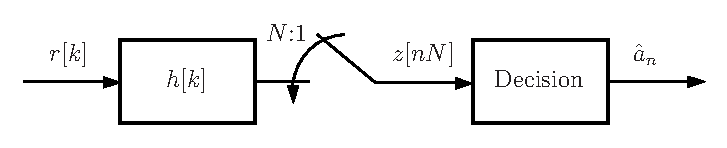
\includegraphics[width=3.75in]{figures/Downsample}
\caption{Downsampling operation.}
\label{fig:Downsample}
\end{figure}




\section{\MakeUppercase{Numerical Results}}
\label{sec:NumericalResults}
\begin{figure}[h]
\begin{center}
\begin{tabular}{ |c|c|c|c|} 
 \hline
 Serial & Naive & Constant Mem & Shared Mem \\ 
 \hline
 129.76 ms & 0.1546 ms & 0.1416 ms & 0.09843 ms\\
 \hline
\end{tabular}\caption{Table of speedup results from individual convolution optimizations}\label{table:convolutionTimes}
\end{center}
\end{figure}
\subsection{Convolution Optimizations}

As seen from the previous table \autoref{table:convolutionTimes}, GPU optimization of convolution was a success! The convolution speedup test involved running convolution on a 720x1280 image witha 5x5 kernel on each of the described methods 10 times, and taking the average of all the attempts for each category. Note that the shared memory implementation is not a standalone implementation. Rather, it is built upon the constant memory implementation as well. 
\begin{figure}[h]
\centering
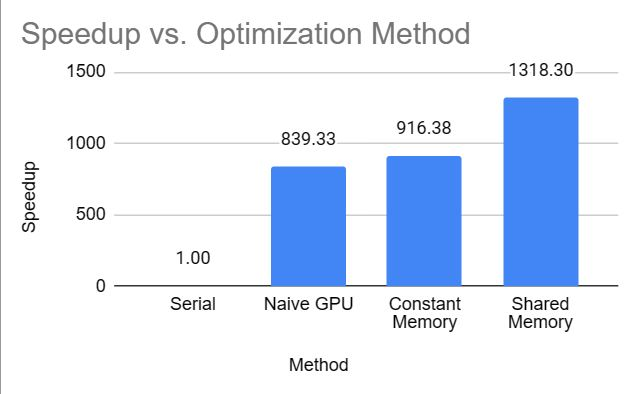
\includegraphics[width=2.5in]{figures/ConvolutionSpeedup}\caption{Speedup amount vs serial implementation.}\label{figure:convolution-speedup}
\end{figure}
Of noteworthiness is the fact that constant memory did not produce the anticipated results. On the naive implementation, each pixel requires 25 global memory reads for the kernel. Multiply that by the total amount of pixels, and a big reduction in global memory reads is achieved. However, performance improvement when compared to a naive GPU implementation was only a 1.09x speedup. The possible reason is that, due to the frequent accesses to memory, data has already been cached. Therefore, constant memory only presented a marginal improvement. 
On the other hand, a shared memory implementation provides a successful improvement, being approximately 1.44x faster than constant memory version. Further performance increase may be obtained by reducing thread divergence, but that was beyond the scope of this project.

\subsection{Histogram Population Optimizations}
As previously stated, the algorithms that were implemented on the GPU include the naive approach, which accesses global memory to retrieve edge pixel information.
The second implementation removes atomic add operations from the inner loops and uses a local accumulator.
The third implementation attempts to load the image into shared memory. However, because of shared memory size constraints, the third implementation was unsuccessful.

\begin{figure}[h]
\begin{center}
\begin{tabular}{ |c|c|c| } 
 \hline
 Serial Implementation & Naive GPU & Local Accumulator \\ 
 \hline
 284362 s & 4.090 s & 4.067 s \\
 \hline
\end{tabular}\caption{Table of speedup results from R-Table Implementations}\label{table:histogramGeneration}
\end{center}
\end{figure}

As seen in \autoref{table:histogramGeneration}, the serial implementation, run on an Intel Core i7 8700k @ 3.7 GHz executed the population of the R-Table in approximately 284.36 seconds.
The first implementation, utilizing the global memory on the GPU using global memory and an atomic add operation within the loop executed the population of the R-Table in approximately 4.090 seconds.
This second implementation on the GPU executed the population of the R-Table in approximately 4.067 seconds.
Speedup from the serial implementation to the naive GPU implementation is 69.5x.
Speedup from the naive GPU implementation to the local accumulator memory is negligible. 
The reason for this being the case has to do with the fact that each thread is tied to one set of parameters at any given time.
Different parameters are being populated by different threads there is no memory contention among atomic operations. 
Changing the algorithm to require less image accesses per thread and instead focusing on populating individual parameters would have been a more fruitful approach to optimizing this step of the HT algorithm.\label{section:histogramGeneration}


\subsection{Streaming}
As mentioned beforehand, streaming was a consideration for a possible performance improvement. While streaming does not increase latency for a single image, it increases overall throughput by pipelining the kernels. The first experiment involves a streaming implementation of all pre-processing kernels, namely Grayscaling, and three convolution kernels, on a set of 60 images. Timing and performance analysis was done, and the throughput measurement includes memory transfer overhead (sending image for kernel operations, and retrieving the output). Here are the results:
\begin{figure}[ht]
\centering
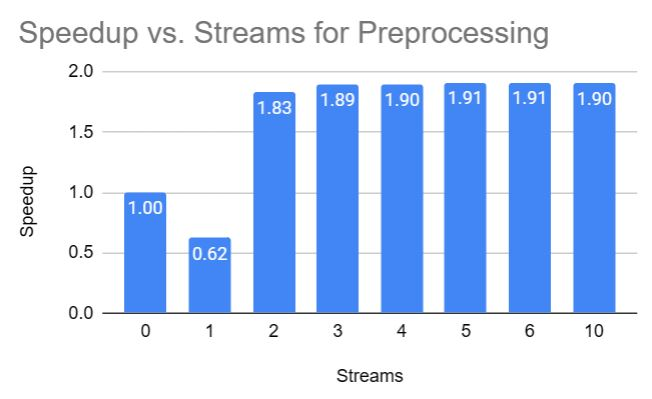
\includegraphics[width=2.5in]{figures/StreamingPreProcessing}\caption{Speedup vs \# of streams for pre-processing}\label{figure:streamPreProcess}
\end{figure}

Seeing the potential success of streaming, the decision was made to create a streaming implementation for the whole algorithm. The initial expectations were that performance improvements would exceed that of the pre-processing speedups. As such, a secondary experiment was realized with the entire process streamed, the entire algorithm with 30 images was executed 10 times for each stream amount.

\begin{figure}[H]
\centering
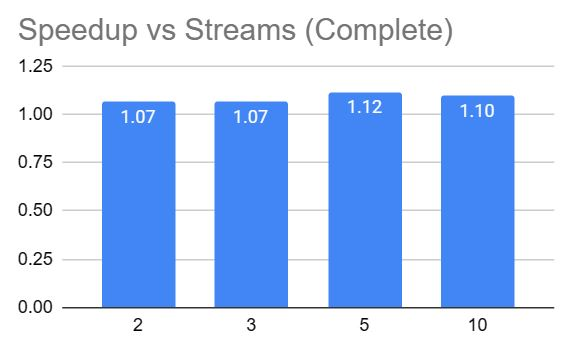
\includegraphics[width=2.5in]{figures/StreamsComplete}\caption{Speedup vs \# of streams for complete process}\label{figure:streamComplete}
\end{figure}

As shown in figure 9, results were not as anticipated. Streaming provided less of a performance improvement than predicted, and by quite a large margin. Upon a root analysis cause, it was determined that the computation time on the Hough Transform far exceeded both pre-processing and memory transfer overhead. Therefore, any performance improvement was largely small in comparison to the Hough Transform. This means that the goal performance of 30 FPS was not met.


\noindent
Once again, you should add sections as needed. Although it is not required, oftentimes a paper will contain some kind of numerical performance results.



\section{\MakeUppercase{Conclusions}}
\label{sec:Conclusions}
\noindent
Examining the execution times for the HT implemented on a serial system shows that while circle detection is possible when serially executed, performance is not sufficient for real time applications.
Implementing a GPU to execute circle detection in an image allows for much faster execution, that, while in its current form is not real-time, can be optimized to execute faster at the cost of accuracy. Convolution and streaming implementations were a major success. However, the Hough Transform implementation was a bigger bottleneck than anticipated. After only achieving a FPS of about 5, the goal of 30 FPS was not reached. There are, however, various signs that this is achievable.
Future work involves implementing different algorithms to populate the R-Table in a more memory access efficient manner using the algorithm discussed in method. 
With the introduction of streaming, batching of images is possible, leading to higher throughput for the image pre-processing steps. We believe this will improve performance significantly, both due to the reduction in kernel launch overhead, as well as freeing up the main bottleneck, which is shared memory constraints.
% This is where you give your final word on what you have written. Now that you have completely developed everything, you want to make sure the reader understands its value and how they benefit from it. You might also connect your paper's findings to a larger context, suggest the implications of your findings, suggest future work, or revisit your paper's original question with the new insights you have presented.



\bibliographystyle{ieeetr}
\bibliography{references}
\end{document}
